\documentclass[a4paper, 12pt]{article}
\usepackage[isolatin]{inputenc}
\usepackage[normalem]{ulem}
\usepackage{graphicx}
\usepackage{cite}

\begin{document}

\subsection{Polynomial Encoding}

The chromosome coding will as follow:
\begin{enumerate}
\item an initial segment detailing which monomials are active (the 1st monomial is always active), these are represented in unary description
\item the chromosome is split into `max.monomials` sets of bits of equal size 
  (a monomial)
\item each monomial is split into `n.vars` sets of `max.degree` size each, i.e., a variable
\item for each variable, the remaining bits give the binary description of the variable degree, i.e., the maximum exponent is given by $2^max.degree-1$
\end{enumerate}

Eg: consider polynomial $x_1^3 x_3 + x_3^7 + x_1 x_2$ with max.monomials = 4, n.vars = 3 and max.degree=3. One possible encoding would be:

$$110 - 011,000,001~~;~~000,000,111~~;~~001,001,000~~;~~110,010,101$$

(for reading purposes the semicolons separate monomials, the commas separate variables)

The first 3 bits inform that the second and third monomials are active while the fourth is not (as said, the first monomial is always active). This last monomial does not enter neither in the polynomial regression nor in the fitness evaluation. However, it acts as a kind of junk DNA, becoming active when the third bit of the entire sequence flips from 0 to 1.

Let's interpret the first monomial description, $011,000,001$. It is divided by three since n.vars=3. The first triple $011$ is the binary description of the exponent of variable $x_1$ which is 3, so the first monomial includes $x_1^3$. The second triple, $000$, means that $x_2$ is not part of the monomial. The thrid triple $001$ says that variable $x_3$ has exponent $1$, so the first monomial consists of $x_1^3 x_3$. All the remaining sets of $9$ bits are interpreted the same way and we get the previous polynomial.

Notice that all binary descriptions give rise to valid polynomials. However, if the coding consists of entirely zeros, by convention, it describes polynomial $x_1$. This has to do with the execution of the polynomial regression that would fail if we interpret it as the zero polynomial. Anyway, for progressive larger  binary descriptions, the chances of getting this zero description decrease exponentially, so it does not impact in any meaningful way in the algorithm's performance.

Somewhat unexpectedly after some experiences it was found that lower values for $\lambda$ sometimes provide better, even if marginal, results. The next figure shows results for the Abalone dataset with five runs for each $\lambda$ (cf. Experimental Results section for more info on this dataset).

\begin{figure}[htb]
	\begin{center}
		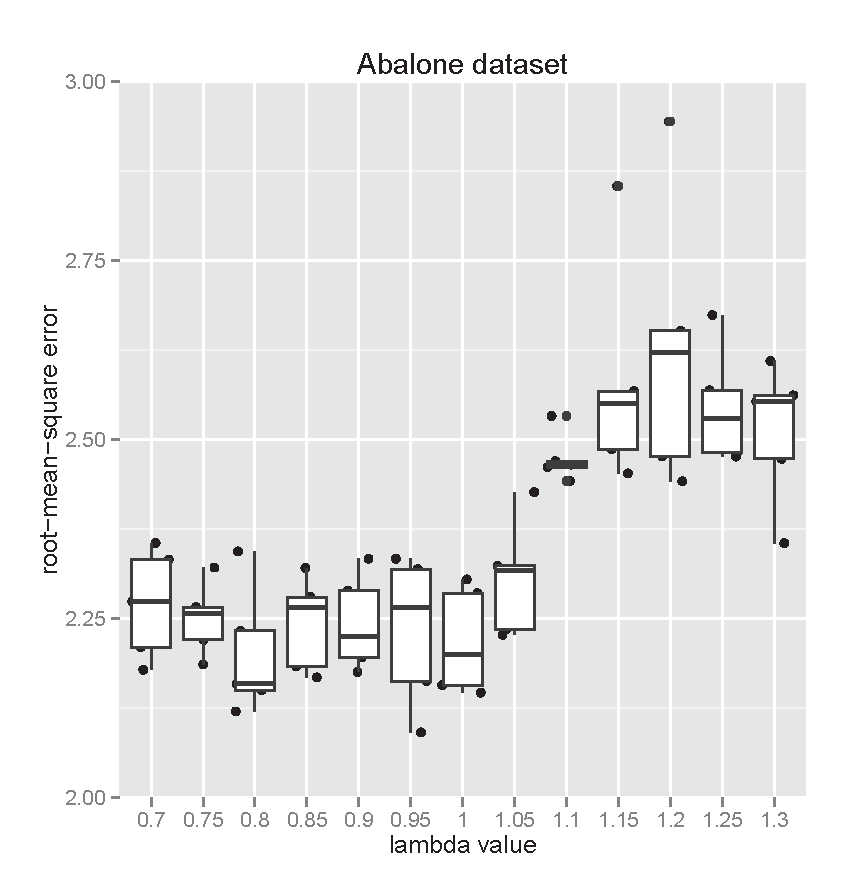
\includegraphics[height=6cm,width=10cm,angle=0]
			{figures/Abalone_dataset_lambdas.eps}
		\caption{fitness progress for Abalone dataset}
	\end{center}
\end{figure}

The values for another dataset:

\begin{figure}[htb]
	\begin{center}
		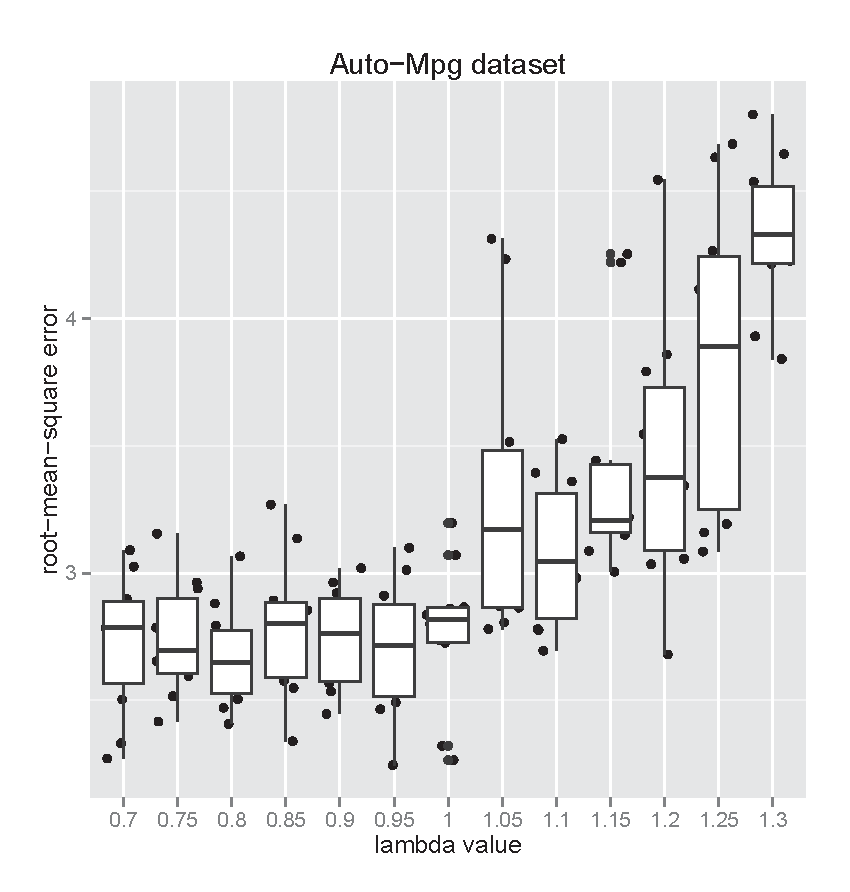
\includegraphics[height=6cm,width=10cm,angle=0]
			{figures/Auto-Mpg_dataset_lambdas.eps}
		\caption{fitness progress for Abalone dataset}
	\end{center}
\end{figure}

The inflection point is around $\lambda = 0.8$. We'll use the regularisation parameter with this value.

\subsection{Regularization}

The polynomial fitness considered so far is based on the ability to predict the test set after the polynomial regression has found the appropriate coefficients $\theta_i$ for each one of the polynomial's monomials $m_i$.

This fitness function tends to prefer more complex polynomials, namely in the number of monomials which provides the regression algorithm for more fitting possibilities. One way to balance this is to provide a regularization term into the fitness function. Our proposal is to include a multiplicative factor into the fitness function proportional to the number of monomials. Thus, the fitness function becomes,

$$
J_{fit}\left( \Theta; D \right) = \lambda^{M} \sqrt{ \frac{1}{n} \sum_{i=1}^n \left( y^{(i)} - h_{\Theta}\left(x_1^{(i)}, \ldots, x_m^{(i)}\right) \right)^2 }
$$

where M is the number of monomials the polynomial has. A $\lambda$ greater than one punishes polynomials with more monomials.

\section{Experimental Results}

These results were found using R's programming language~\cite{R}.

To compare this paper's algorithm we applied the exact same train and test samples with other learning algorithms, namely: Linear Regression, Support Vector Machines~\cite{Meyer12}, Regression Trees~\cite{Therneau13}, Conditional Inference Trees~\cite{Hothorn06}~\cite{Strobl07}~\cite{Strobl08} and Random Forests~\cite{Liaw02}

In order to train and test the performance of GApoly it was used several datasets (see below). For each dataset, we selected 70\% for training purposes and the remaining observations to make the test set in order to compute the estimated rmse. To achieve more robust results, for most datasets there were 25 runs, each one with different samples for the train and test sets. For the datasets with attribute values of different magnitudes, a preliminary scaling was executed. The results below are boxplots for the test set error predictions over these different runs.

\textbf{Artificial}: this is an artificial dataset with four numeric features, $x_1, \ldots x_4$, where $x_1,x_3$ are outcomes from Poisson random variables, and $x_2,x_4$ from Normal random variables. The dependent variable $y$ is given by expression $x_2x_4^2 + x_1^2x_3 + 5$. The dataset includes 50 observations. 

\begin{figure}[htb]
	\begin{center}
		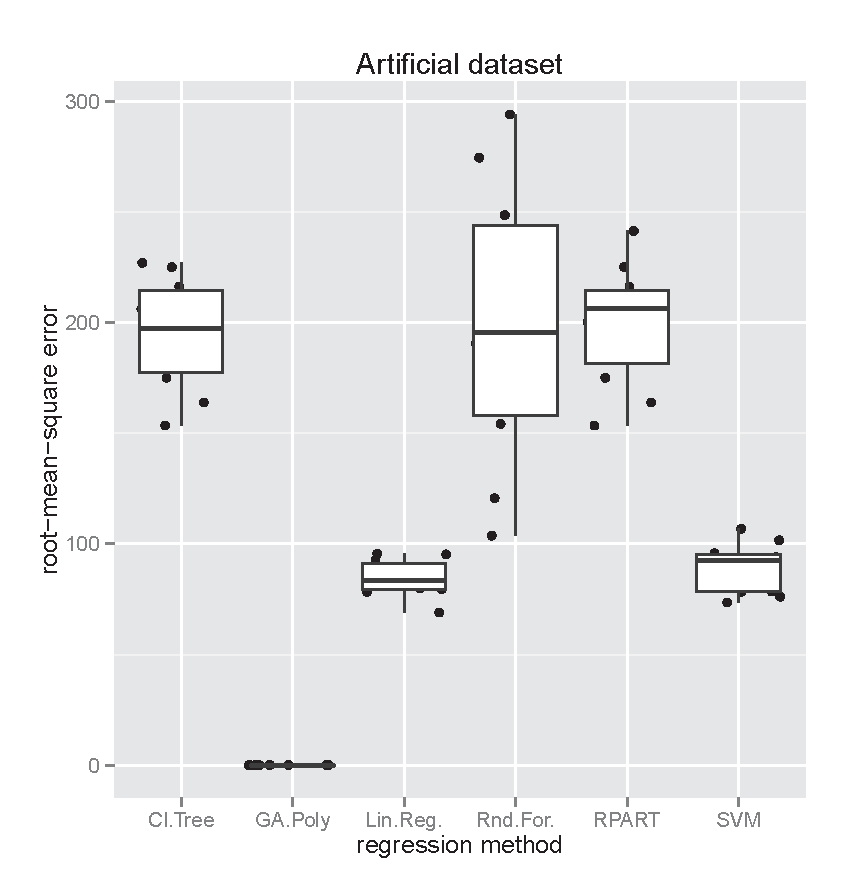
\includegraphics[height=6cm,width=10cm,angle=0]
			{figures/artificial_dataset1_lambda1.0.eps}
		\caption{results for Artificial dataset}
	\end{center}
\end{figure}

This dataset was used in order to verify if GApoly was able to find the polynomial relation, which the algorithm did. In this case, all runs used a population of 100 with 50 iterations for each run.

In the next datasets, the population was 250 with 100 iterations for each run

\textbf{Housing}: This data set concerns the task of predicting housing values in areas of Boston. There are 13 continuous attributes and the dependent variable is the median value of owner-occupied homes in \$1000's\footnote{This and the remaining regression datasets were selected from Luis Torgo's data repository, http://www.dcc.fc.up.pt/~ltorgo/Regression/DataSets.html. Most of these set originally come from UCI ML repository, http://archive.ics.uci.edu/ml/}. There are 506 observations.

\begin{figure}[htb]
	\begin{center}
		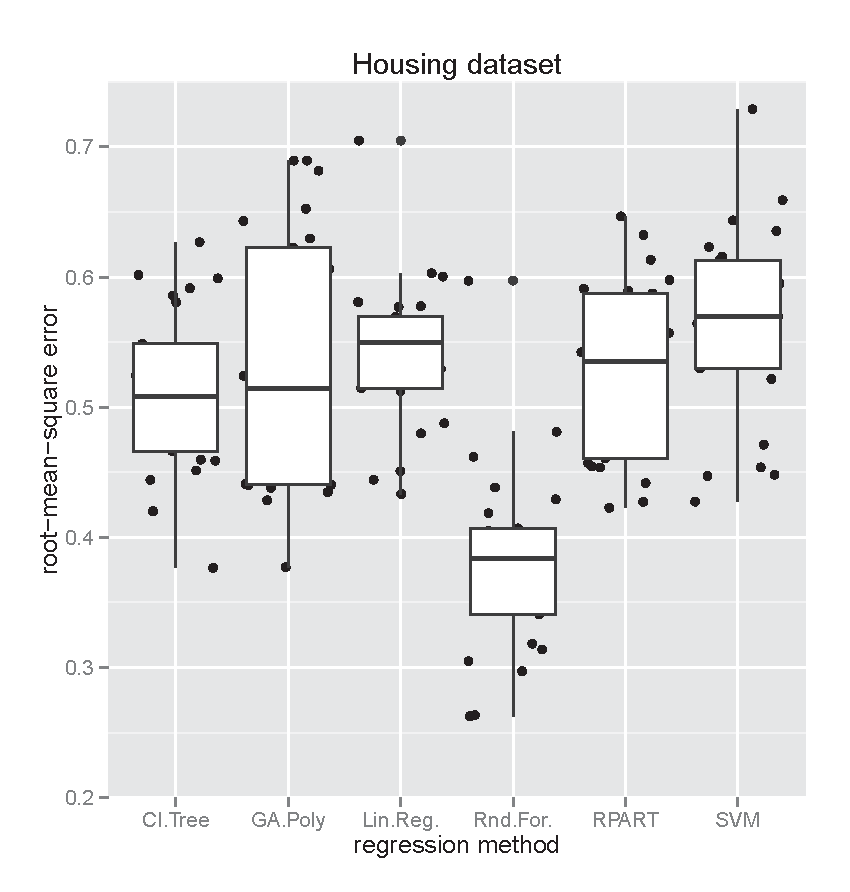
\includegraphics[height=6cm,width=10cm,angle=0]
			{figures/Housing_dataset_lambda0.8_25runs.eps}
		\caption{results for Boston Housing dataset}
	\end{center}
\end{figure}

Just as an example of the model the GApoly algorithm outputs: in this dataset the best polynomial, with a rmse of 0.38 for the test set, was the following:

$$y = -0.12 x_6 x_9^4 + 0.78 x_6 - 0.4 x_9^2 x_{13} + 0.17 x_{13}^2 - 0.044$$

where the attributes mean:
$x_6$, RM average number of rooms per dwelling;
$x_9$, RAD index of accessibility to radial highways;
$x_{13}$, Lower status of the population.

\textbf{Abalone}: This dataset can be used to predict the age of a abalone shell using the given 8 numeric attributes concerning several physical measurements. There are 4177 observations.

\begin{figure}[htb]
	\begin{center}
		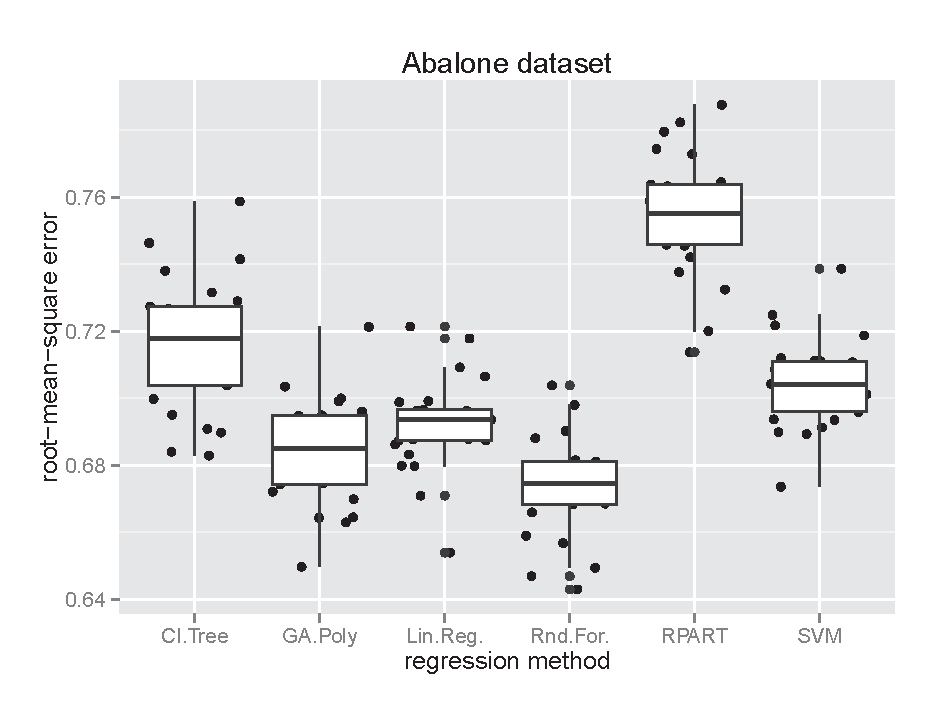
\includegraphics[height=6cm,width=10cm,angle=0]
			{figures/Abalone_dataset_lambda0.8_25runs.eps}
		\caption{results for Abalone dataset}
	\end{center}
\end{figure}

% best polynomial, rsme 0.65
% $$y = 0.52 s_1^2 x_5 - 0.13 x_2 x_8 -0.75 x_1^2 x_6 + 0.78 x_8 + 0.18 $$

\textbf{Auto-MPG}: This dataset is used to predict fuel consumption in miles per gallon, based on two discrete and five continuous attributes. There are 398 observations. Here are the initial observations:

\begin{figure}[htb]
	\begin{center}
		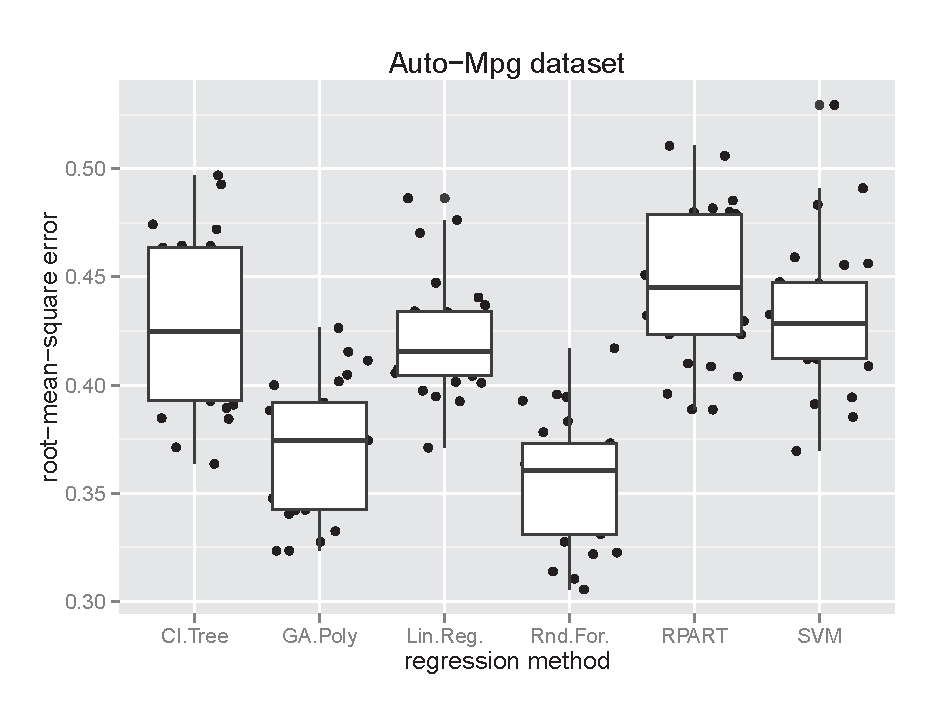
\includegraphics[height=6cm,width=10cm,angle=0]
			{figures/Auto-Mpg_dataset_lambda0.8_25runs.eps}
		\caption{results for Auto-MPG dataset}
	\end{center}
\end{figure}

% best polynomial, rmse 0.32
%$$ y = 0.4 x_6 + 0.02 x_5^3 x_6 - 0.85 x_4 + 0.23 x_4^2 - 0.26 $$

\textbf{Kinematics}: This dataset is concerned with the realistic simulation of the forward kinematics of an 8 link robot arm. The task is to predict the distance of the end-effector from a target using 8 continuous attributes. There are 8192 observations.

\begin{figure}[htb]
	\begin{center}
		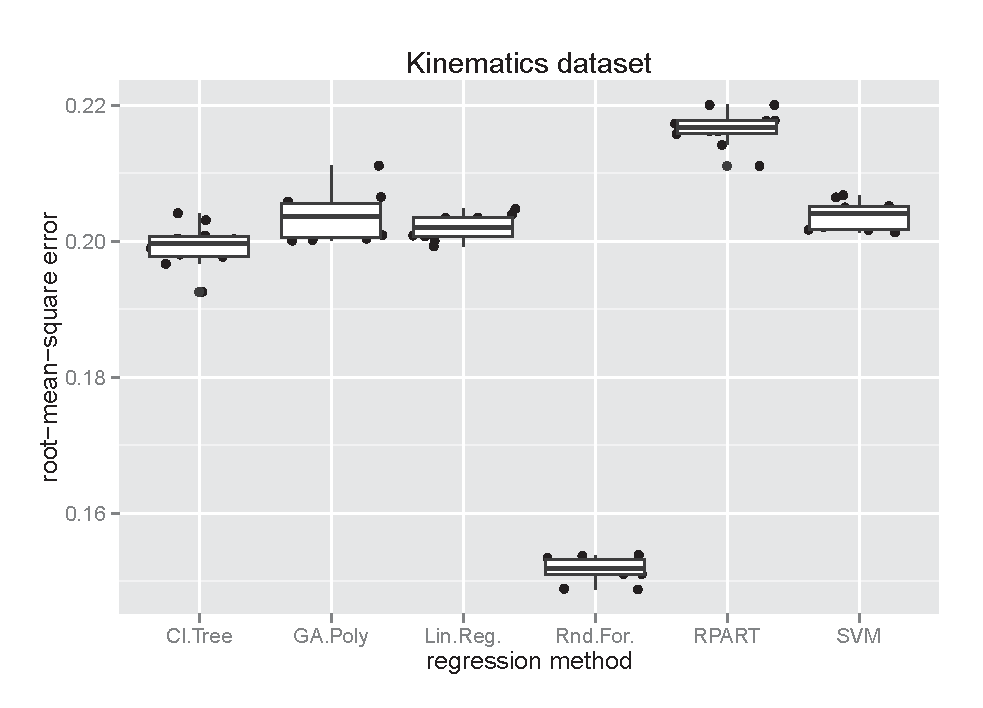
\includegraphics[height=6cm,width=10cm,angle=0]
			{figures/Kinematics_dataset_lambda1.0.eps}
		\caption{results for Kinematics dataset}
	\end{center}
\end{figure}

\subsection{Convergence speed}

The GA quickly proceeds in the first 50 to 100 generations to reasonable error rates. Then, it proceeds slower achieving best solutions with marginal error reduction. Since the entire learning process takes some time, in the current R implementation\footnote{the processing time can probably be speeded by one to two orders in magnitude if the process is implemented in a low level programming language like C++. However, speed optimisation was not the focus of this article}, placing a limit between 50 to 100 generations already achieves good results, relative to higher iteration values. The next figure shows a typical error evolution for the dataset Abalone given two different values for $\lambda$.

\begin{figure}[htb]
	\begin{center}
		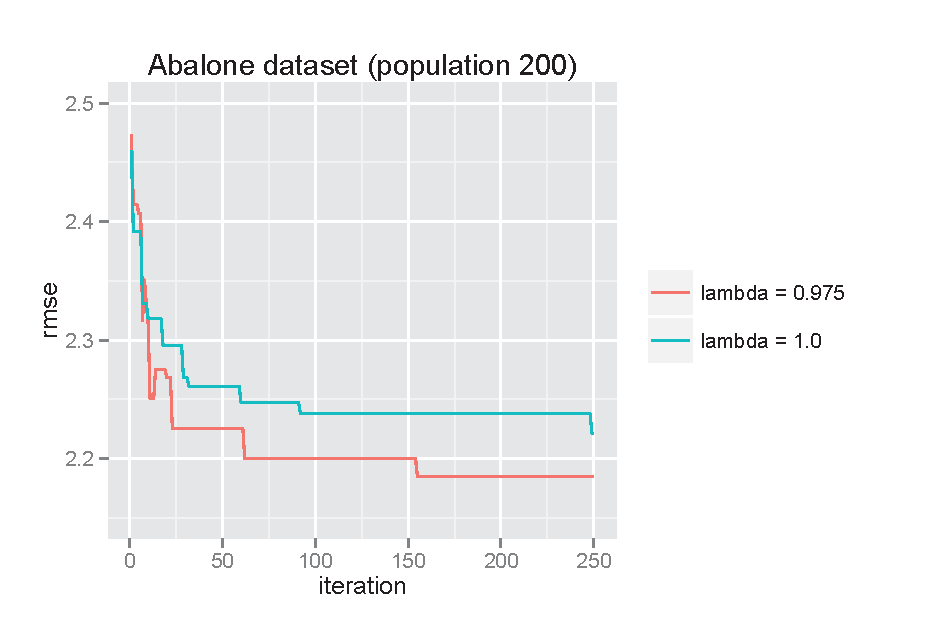
\includegraphics[height=6cm,width=10cm,angle=0]
			{figures/Abalone_fitnessProgress.eps}
		\caption{fitness progress for Abalone dataset}
	\end{center}
\end{figure}

Somewhat unexpectedly after some experiences it was found that lower values for $\lambda$ tend to provide better, even if marginal, results. The next figure shows results for the artific

\subsection{Discussion}

The proposed method has competitive results comparing with some well-known regression methods. Only Random Forest outperforms GApoly systematically (it outperforms all the others) except in the Auto-MPG test and, of course, in the artificial dataset that uses a straightforward polynomial relation. 



\section{Bibliography}

\bibliographystyle{plain}
\bibliography{mybib}

\end{document}

